\chapter{Results} 
\label{ch:results}
This chapter presents and describes the results of the conducted performance evaluation of the context-based authentication protocol and group-key management protocol. 

\section{Performances of the authentication scheme}
In this project two different fingerprints are proposed: one based on the ambient data from the sensors and one based on the recorded audio.
The similarity of these fingerprints is then used to decide if devices can establish a connection by using a key generated from fuzzy commitment scheme.

The fingerprint length generated from the ambient data is 320 bits long and required 1000 data from each sensor, which means that the device has to acquire data for 10000 seconds.
The features used to generate this fingerprint are: temperature, humidity, gas, light and  pressure.
For the analysis have been used only the parameters which were correlated among the devices during the time and the ones obtained from the gyroscope and accelerometer were completely discorrelated.
A fingerprint 64-bit long is generated from each feature and then they have been combined in order to generated a unique 320 bit long fingerprint.

The fingerprint generated from the recorded audio has a length of 512 bits and required 10 seconds of audio recording.
In Table \ref{tab_sensorAcc} and Table \ref{tab_audioAcc} are shown the performances of the two fingerprints while changing the number of different bits $t$ between 2 different fingerprints.

The analysis is performed comparing fingerprints from the same environment but in different times in order to verify if the scheme is able to identify if two fingerprints are generated in different periods.
In the tables are shown the following parameters: 
\begin{itemize}
    \item the amount of authenticated true claims (T.A.) 
    \item the amount of not authenticated false claims (T.R.)
    \item the amount of authenticated false claims (F.A.)
    \item the amount of not authenticated true claims(F.R.)
\end{itemize}

\begin{table}[H]
\label{tab_sensorAcc}
\begin{center}
\begin{tabular}{|c|c|c c c c|}
\hline
&\multicolumn{5}{c|}{\textbf{Sensors}} \\\cline{2-6}
\textbf{Environment} & \textit{t} &\textbf{T.A.}& \textbf{T.R.} & \textbf{F.A.}& \textbf{F.R.} \\ \cline{1-6}
\multirow{4}{*}{Factory}
& 50 & 1 & 1071 & 0 & 104 \\ \cline{2-6}
& 80 & 18 & 1065 & 6 & 87 \\ \cline{2-6}
& 92 & 46 & 1059 & 12 & 70 \\ \cline{2-6}
& 100 & 55 & 1055 & 16 & 50 \\ \cline{1-6}
\multirow{4}{*}{Lab}
& 50 & 0 & 525 & 0 & 70 \\ \cline{2-6}
& 80 & 5 & 525 & 0 & 65 \\ \cline{2-6}
& 92 & 20 & 525 & 0 & 50 \\ \cline{2-6}
& 100 & 36 & 519 & 6 & 34 \\ \cline{1-6}
\end{tabular}
\caption{Accuracy results of the fingerprints generated from the sensors data changing the parameter $t$.  }
\end{center}
\end{table}

\begin{table}[H]
\label{tab_audioAcc}
\begin{center}
\begin{tabular}{|c|c|c c c c|}
\hline
&\multicolumn{5}{c|}{\textbf{Audio}} \\\cline{2-6}
\textbf{Environment} & \textit{t} &\textbf{T.A.}& \textbf{T.R.} & \textbf{F.A.}& \textbf{F.R.} \\ \cline{1-6}
\multirow{4}{*}{Factory}
& 190 & 54 & 151 & 369 & 21 \\ \cline{2-6}
& 180 & 39 & 254 & 266 & 36 \\ \cline{2-6}
& 170 & 16 & 362 & 158 & 59 \\ \cline{2-6}
& 160 & 6 & 434 & 86 & 69 \\ \cline{1-6}
\multirow{4}{*}{Lab}
& 180 & 9 & 12 & 238 & 1 \\ \cline{2-6}
& 170 & 44 & 44 & 206 & 6 \\ \cline{2-6}
& 160 & 32 & 82 & 168 & 18 \\ \cline{2-6}
& 150 & 18 & 123 & 127 & 32 \\ \cline{1-6}
\end{tabular}
\caption{Accuracy results of the fingerprints generated from the recorded audio changing the parameter $t$. }
\end{center}
\end{table}

In the factory's use case, the device  located far from the others is considered in a different environment.
The results show how difficult is to recognize fingerprints generated in different time periods. 
In Table \ref{tab_rejectionAudio} and Table \ref{tab_rejectionSensor} has been applied the fuzzy commitment scheme between devices located in different environments.
The tests are performed changing the parameter $t$ used by the error correcting code scheme.

The results show that when two devices are located in different environments, they produce dissimilar fingerprints and even with high values of $t$, it results difficult to authenticate them.
In fact, using an error correcting code able to correct the 35 \% of the message in the case of audio fingerprints and 37\% in the case of the fingerprint generated by the other ambient features, the scheme authenticate devices in different environments the 13.3 \% and 12.3\% of the cases respectively.

\begin{table}[H]
\label{tab_rejectionSensor}
\begin{center}
\begin{tabular}{|c|c c c|}
\hline
\multicolumn{4}{|c|}{\textbf{Sensors}} \\\hline
\textit{t} &\textbf{False Authenticated}& \textbf{True Rejected}& \textbf{Error Rate (\%)}  \\ \cline{1-4}
130 & 534 & 1181 & 31.1\\ \cline{2-4}
120 & 211 & 1504 & 12.3\\ \cline{2-4}
110 & 60 & 1655 & 3.5\\ \cline{2-4}
100 & 12 & 1703 & 0.7\\ \cline{2-4}
90 & 0 & 1715 & 0 \\ \cline{1-4}
\end{tabular}
\caption{Authentication using fingerprints generated from the sensors data by devices located in different environments. }
\end{center}
\end{table}

\begin{table}[H]
\label{tab_rejectionAudio}
\begin{center}
\begin{tabular}{|c|c c c|}
\hline
\multicolumn{4}{|c|}{\textbf{Audio}} \\\hline
\textit{t} &\textbf{False Authenticated}& \textbf{True Rejected}& \textbf{Error Rate (\%)}  \\ \cline{1-4}
180 & 116 & 759 & 13.3\\ \cline{2-4}
170 & 75 & 800 & 8.6\\ \cline{2-4}
160 & 49 & 826 & 5.6\\ \cline{2-4}
150 & 20 & 855 & 2.3\\ \cline{2-4}
140 & 4 & 871 & 0.5\\ \cline{2-4}
130 & 0 & 875 & 0\\ \cline{1-4}
\end{tabular}
\caption{Authentication using fingerprints generated from the recorded audio by devices located in different environments. }
\end{center}
\end{table}

\section{Lightweight protocol}
 In this section is presented the performance results of the proposed scheme comparing it with the scheme designed in \cite{Porambage2015}
In order to perform the performance evaluation, the environment is set.
The evaluation is done for a sensor network consists of 5 nodes and 1 gateway. 
The experiment setup is described as follows:
\begin{itemize}
    \item[Cooja] The measurement is performed using Cooja. By using Cooja, it is easier to return to a certain initial condition and perform the measurement. Initially, 5 Tmote Sky nodes and one Gateway  are added in the simulation environment. The Radio Messages are shown so the traffic can be observed. The Cooja interface is shown in Figure \ref{fig_cooja}.
    \item[Energest] Energest is a built-in tool used to count the number of CPU ticks consumed for performing certain task. The number of ticks is correlated to energy consumption and processing time.
\end{itemize}
\begin{figure}[!h]
\centering
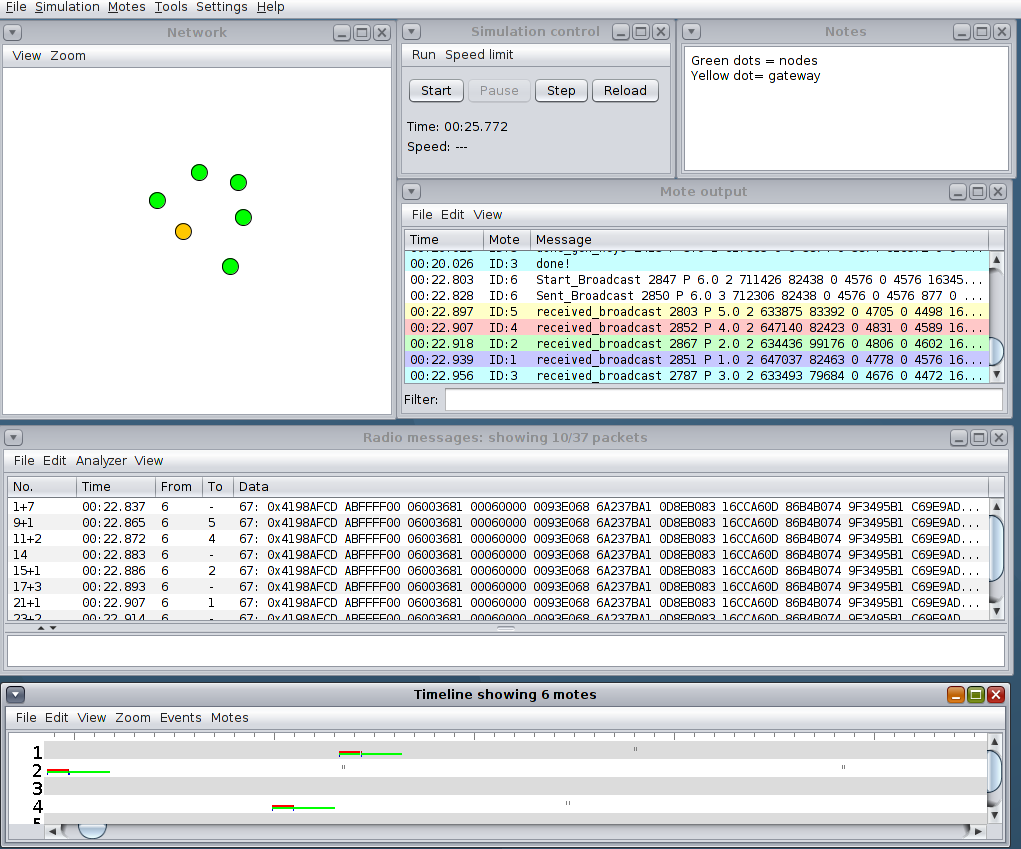
\includegraphics[width=6in]{images/cooja.png}
\caption{Cooja User Interface.}
\label{fig_cooja}
\end{figure}

The storage overhead analysis explains the memory utilized to store the parameters used by the protocol. 
The energy analysis is based on the estimate energy consumption of the computation and communication energy cost of the protocol.
Security analysis explains how the commons security threats are mitigated in the proposed solution.

\subsection{Storage Overhead}
The amount of memory required to store security parameters and key space is considered the storage cost. The total number of devices in the network is $d = m + 1$ , which is the number of nodes $m$ plus the gateway $G$. 
Calculations are performed for the \textit{secp192r1} curve ECC operations, estimating the dimension of an EC point $P = ((P_x),(P_y))$ of 48 byte.

The storage overhead slightly varies and depends on the role of the device in the network. 
In Table \ref{resourceNode} and Table \ref{resourcesGateway} are shown the parameters needed by the nodes and the gateway respectively. 
The parameters are considered using the \textit{secp192r1} elliptic curve and do not include the ones used by the authentication protocol.
Each node requires 147 bytes while the gateway has more overhead depending on the number of nodes  $n$ in the group for a total amount of $121 + 26 n$ bytes.

\begin{table}[H]
\caption{Space utilized by each parameter stored in the node using \textit{secp192r1} curve }
\label{resourceNode}
\begin{center}
\begin{tabular}{|c||c|}
\hline
 \textbf{Resource} & \textbf{Dimension (Bytes)}\\
\hline
\textit{Public Key} & 48\\
\hline
\textit{Private Key} & 24\\
\hline
\textit{Group ID} & 1\\
\hline
\textit{Shared Secret (with gateway)} & 24\\
\hline
\textit{Group Secret} & 24\\
\hline
\textit{MSK} & 24\\
\hline
\textit{Gateway's address}  & 2\\
\hline
\end{tabular}
\end{center}
\end{table}

\begin{table}[H]
\caption{Space utilized by each parameter stored in the gateway using \textit{secp192r1} curve }
\label{resourcesGateway}
\begin{center}
\begin{tabular}{|c|c|}
\hline
 \textbf{Resource} & \textbf{Dimension (Bytes)}\\
\hline
\textit{Public Key} & 48\\
\hline
\textit{Private Key} & 24\\
\hline
\textit{Group ID} & 1\\
\hline
\textit{Shared Secrets (with nodes)} & $24 \times n$\\
\hline
\textit{Group Secret}  & 24\\
\hline
\textit{MSK} & 24\\
\hline
 \textit{Nodes'  addresses} & $2 \times n$\\
\hline
\end{tabular}
\end{center}
\end{table}


\subsection{Energy Consumption Analysis}
%%%%%%%%%%%%EDIT
The performance analysis represents a major concern at this time and it is based on two key factors: the estimated energy consumption of the computation and communication energy cost of the protocols.
For the potential enormous number of IoT devices, this will help saving the energy significantly in a long term. 
For disposable-battery-powered devices, using efficient protocol means changing battery less often, which is a challenge faced by some kind of devices (i.e., devices deployed in hazardous environments or in location difficult or impossible to access frequently). 
This helps reducing battery consumption which should be recycled in certain way.
The energy consumption for each phase is calculated as follows:
%%%%%%%%%%%%%%
\begin{center}
    $energy\_consumption=\frac{Energest\_value \times current \times voltage}{RTIMER\_SECOND \times runtime}$
\end{center}

where \textit{RTIME\_SECOND} represents the number of clock ticks per second, and the values of the current and voltage are obtained from the datasheets as shown in Table \ref{tmote}.
The \textit{Energest\_Value} is the number of  MCU clock ticks (in this case: \textit{MSP430} ) required to perform common tasks like CPU usage and messages transmission or reception. 

\begin{table}[H]
\caption{Energy consumption and duration for each step of the protocol using \textit{secp192r1} curve ECC operations .}
\label{energyTime}
\begin{center}
\begin{tabular}{|c|c|c|}
\hline
& \textbf{Energy (mJ)} &  \textbf{Duration (s)}\\
\hline
\textbf{ECDH} & 19.02 & 19.220\\
\hline
\textbf{EC Point Multiplication}& 19.02 & 19.199\\
\hline
\textbf{HMAC}& $\approx0$ & 0.010\\
\hline
\textbf{AES Encrypt}& $\approx0$ & 0.010\\
\hline
\textbf{AES Dencrypt}& $\approx0$ & 0.014\\
\hline
\end{tabular}
\end{center}
\end{table}

At the node's side the complete computational overheads remain constant, irrespective of the size of the secure group.
The complete computation energy for the proposed protocol is approximately $112 mJ$ where approximately $52.8 mJ$ are spent for communication purposes. 
In Table \ref{energyTime} is shown how much time and energy are spent during each phase. 

Our protocol consumes around 6.25\% less energy than the \textit{protocol 2} in \cite{Porambage2015}.
Considering two Zinc-carbon AA batteries of 1.5 V nominal voltage and 800 mAh average capacity, the available energy is 8640 J. Consequently, this value correspond to 0.0013\% of the total available energy for one complete execution of our protocol. 
This  implies that the group key establishment phase can be executed around 77143 times.

As shown in Table \ref{energyCons}, the number of operations performed at the node side is less in the proposed protocol than the one compared with.

Compared to other protocols, the proposed one keeps the computation overhead at the node's side constant and not dependent on the number of nodes in the group.
\begin{table*}[h]
\caption{Computational overhead during each step.}
\label{energyCons}
\begin{center}
\begin{tabular}{|c|c|c|}
\hline
 & \multicolumn{2}{c|}{ \bf Node Computation Overhead}\\
\hline
\textbf{Phase} & \textbf{Proposed Protocol} & \textbf{Protocol 2 \cite{Porambage2015}}\\
\hline
 MSK establishment &  $(HMAC \approx 0) + (AES_{D}\approx0) + PM$ & $4PM + 3PA$\\ 
\hline
 Adding new node &  $(HMAC \approx 0) + (AES_{D}\approx0) + PM$ & $4PM + 3PA$\\
\hline
 Removing nodes &  $(AES_{D}\approx0) + PM$ & $4PM + 3PA$\\
\hline
\end{tabular}
\end{center}
\end{table*}

\subsection{Security Analysis}
In the security analysis are considered two type of attacker: passive and active attacker.
A passive adversary is able to only eavesdrop the ongoing communication between the nodes and the gateway trying to learn some useful information and can read all the public parameters.
As explained in Section \ref{theory:ECC}, due to the ECDL assumption is hard to compute private parameters knowing the public ones.
Therefore, learning something useful by eavesdropping the communication results infeasible since a private key is needed to derive a shared secret or the group key.

An active adversary might impose MITM (Man In The Middle) attacks during the key establishment process.
In the proposed schema, MITM attack resistance is provided by including a context-based authentication using a fuzzy commitment scheme.
An attacker, during the key establishment, needs to generate a key $\kappa$ and to use it together with his shared secret $s$ in order to perform a MITM attack. 
In fact, during the key establishment phase, the node which wants to join the group has to include a value generated with $HMAC(\kappa , s)$ , and the gateway will restore that value using his own value $\kappa$.
To generate a valid value $\kappa$ the attacker needs to get similar ambient data to the ones gotten from gateway, which means be located "close" to it.
An approach is to perform a brute force attack in order to get a valid value $\kappa$ but this means that the attacker has to try a prohibitively large number of combinations, since the commitment value is considered a random value.
It is assumed that devices located in the same ambient are considered trusted and then able to participate to the group-key establishment. 

An active attacker might try to illegitimately compute the group secret to fake the membership but, choosing a large prime $q$ for the elliptic curve, this attack is rendered impossible due to the huge amount of points on the curve to test.

In this thesis is not proposed a solution to the physical examination of the nodes from an attacker.
Moreover, the proposed scheme do not provide a solution to denial of service attacks.


